\section{Experiment 1: Quadratic Voting, Likert surveys, and Donation}
We designed a between-subject experiment to answer RQ1 and RQ3. We recruited participants from Amazon Mechanical Turk (MTurk) and divided them into two groups: the Likert group and the QV group. Participants in both groups received compensation once they completed the experiment. The Likert Group received \$0.75, and the QV Group received \$1.75 due to the difference in the length of the study. The goal of a between-subject study is to understand how different the two survey tools yield results independently.

To conduct the comparison of the QV and Likert survey, we ought to collect the participant's true preferences as a baseline. This baseline comes from the amount of donation that participants donated to a charity. We believe that an individual's donation behavior is similar to their attitude of whom they contributed. We believe donation is a suitable task because of the following reasons. First, donation tasks are easily relatable, given that they occurred in real life. Adult individuals regularly exercise monetary behaviors and make financial decisions daily. These characteristics of the donation task mean that participants should not have challenges completing this task. Second, donations are simple to conduct, even on a large scale. It does not require in-person interactions. Third, donation tasks appeared in many experiments \cite{Xiao2019, benz2008people, gendall2010effect} as a valid indicator of participants' behavior. Fourth, donating is a behavior that contains complimentary and homogenous choices, and each of the options is independent. The donation task is a clear example of choosing one out of $K$ in a real-life setting.

\section{Experiment Flow}
\begin{figure}[htpb]
    \centering
    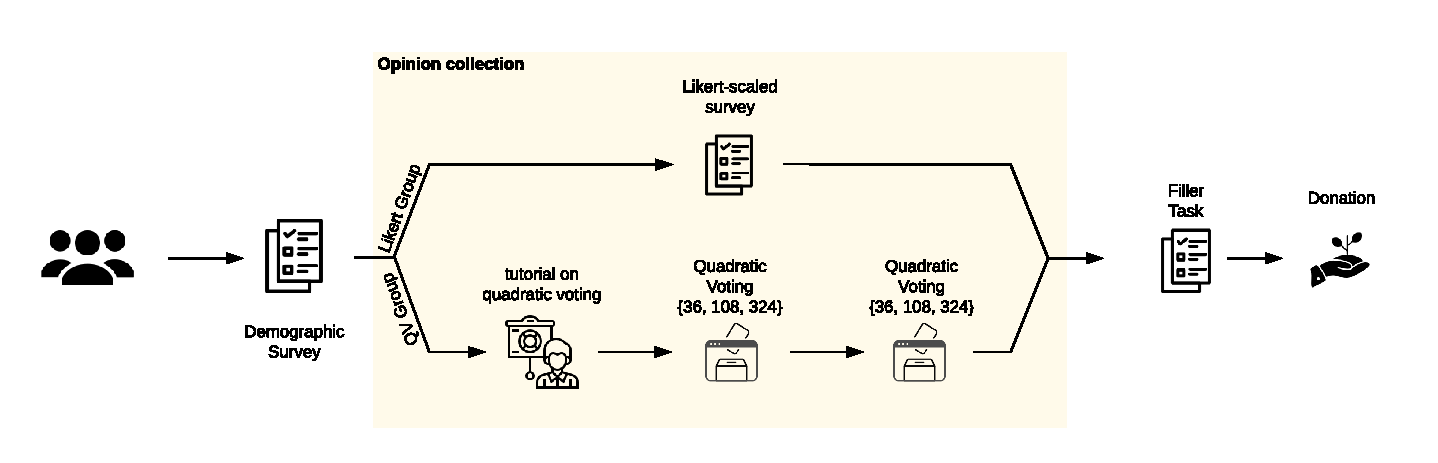
\includegraphics[width=\textwidth, keepaspectratio=true]{content/image/exp1_flow.pdf}
    \caption{
        This experiment conducted between subjects. We divided participants into two groups. Participants that took the upper path were in the Likert Group, who expressed their attitudes toward various social causes through a five-point Likert Survey. The alternative was the QV group who replied attitudes through two QV surveys, each with a different combination among the three possible votes: $36$, $108$, or $324$ credits.
    }
    \label{fig:exp1_image_flow}
\end{figure}

We summarize the experiment procedure in \Cref{fig:exp1_image_flow}. The experiment consisted of four steps: Participants filled out the demographic survey as the first step. Based on the demographics, participants completed one or more surveys, as highlighted in the figure. Participants in the Likert group filled out one Likert survey, while participants in the QV group completed two QV surveys. After that, participants filled out another survey, the distraction survey, to divert their attention before completing the final task. We ask participants to donate to a list of charities. We explain each of these steps in detail.

Before starting the experiment, we told participants in the consent form that this study aimed to understand their opinions on several social causes and required them to complete a donation task. Participants completed a demographic survey after confirming the consent form. We collected the participant's gender, ethnicity, age range, household income level, education level, and current occupation. Based on the age and education level, we divided participants into seven groups and ensured that each group contained similar distribution as to the 2019 United States census. This experiment further categorized into seven groups: the Likert Group (Group 1) and the QV Group (Group 2 to Group 7).\par

The Likert Group, shown as the upper path in the shaded area of \Cref{fig:exp1_image_flow}, expressed their opinion using a Likert survey. The QV Group, shown as the lower path in the shaded area of \Cref{fig:exp1_image_flow}, revealed their opinions by completing two QVs, each with a different number of voice credits. We divided the QV Group into six subgroups to answer research question three, which, investigated how the number of voice credits impacted the survey results.Participants were randomly assigned to two voice credits from three possible values: $N \times O$, $N^{1.5} \times O$, and $N^2 \times O$. Here, $N$ is the number of options in the survey, and $O$ is the number of levels excluding neutral on the Likert survey. In this experiment, participants answered their opinion to $9$ societal causes, therefore $N=9$. We used a five-point Likert survey, which translated to $O=4$. Thus, the three possible voice credits in the experiment were $36$, $108$, and $324$. With these three possible values, each of the six subgroups represented a combination of any two voice credits.\par

We knew that a voice credit too little will bar participants from expressing their opinion. Therefore, we want to make sure that even with QV that had the lowest voice credit, participants can strategically express the same result in QV as if they were in Likert. Given that we used a 5-point Likert scale in the experiment, which the participant can select up to ``very agree''  or ``very disagree'', the participant would need at least four voice credits to express the same level of responses in a QV scenario. Participants do not need to use all their voice credits, so the maximum amount of voice credit participants need to express any combination of the response of a Likert is $N \times O$. To test how larger voice credits impacted people's choices, we set an exponential increase based on the number of options on the survey that changed from power of $1$, $1.5$ to $2$.\par

For the Likert group, the survey looked identical to a typical five-point Likert survey. We assumed that participants had prior knowledge in Likert surveys. Participants were presented with the nine societal causes, and were asked the importance each of these causes: With options ranging from ``Very important'' to ``Very Unimportant.''

For the QV group, we asked participants to watch a prerecorded tutorial video of QV's concept and how to operate the QV interface. The experiment allowed participants unlimited time to interact with a demo QV interface to make sure that they were comfortable working with QV. This process is what the ``tutorial on quadratic voting'' stands for in \Cref{fig:exp1_image_flow}. To ensure that participants paid attention to the video and understood QV, we asked participants to answer a quiz containing five multiple-choice questions. They would continue with the survey if they answered at least three questions correctly. Once participants passed the quiz, participants will encounter a QV with either 36, 108, or 324 voice credits. They vote in QV using these voice credits on the nine identical options presented to the Likert Group. Participants would repeat this action using a different voice credit. We show these two QV surveys as two QV icons in \Cref{fig:exp1_image_flow}.

After both groups of participants completed their surveys in the opinion collection stage, they finished a short answer question asking their thoughts related to another set of societal issues. These societal issues in this survey were unrelated to any presented in the previous stage. We designed this survey to distract participants intentionally. We do not want participants to connect their survey responses directly to their behaviors in the donation task.

The last step of this experiment was asking participants to complete a donation task. This task presented participants with nine organizations, each referring to one of the nine societal causes that we listed during the opinion collection phase. Participants could donate any amount to any of the organizations listed on the donation page as long as the total donation value did not exceed \$$35$ dollars. While participants did not donate out of their pocket, to ensure incentive compatibility, we designed a mechanism so that participants did not donate imaginatively. Participants were aware that everyone in $70$ participants would win $35$ U.S. dollars. Assuming winning the \$$35$ U.S. dollars, we asked participants if they would want to donate some money to any of the nine charity groups. Participants are also aware that they keep the remaining amount of undonated cash if they win the lottery. Further, participants were aware that the research team would match one dollar to each dollar they donated to an organization if they won the lottery. This setup meant that the donation behavior carried an underlying cost.

To minimize the difference across groups in the study, we used the same prompt across the Likert survey, QV, and the donation task. We explicitly told the participants that there are limited resources in society, and people have different preferences at allocating resources. We asked the participants, 
``What societal issues need more support?'' across all our surveys.

To ensure that the nine societal causes covered a broad spectrum of categories. We used the categorization of charity groups on Amazon Smile, a popular donation website that has accumulated over 100 million dollars of donations, as our topics of the societal causes. The categories include:
\begin{enumerate}[label={},leftmargin=\parindent]
    \item (1) Pets and Animals: Animal Rights, Welfare, and Services; Wildlife Conservation; Zoos and Aquariums
    \item (2) Arts, Culture, Humanities: Libraries, Historical Societies, and Landmark Preservation; Museums; Performing Arts; Public Broadcasting and Media
    \item (3) Education: Early Childhood Programs and Services; Youth Education Programs and Services; Adult Education Programs and Services; Special Education; Education Policy and Reform; Scholarship and Financial Support
    \item (4) Environment: Environmental Protection and Conservation; Botanical Gardens, Parks and Nature Centers
    \item (5) Health: Diseases, Disorders, and Disciplines; Patient and Family Support; Treatment and Prevention Services; Medical Research
    \item (6) Human Services: Children's and Family Services; Youth Development, Shelter, and Crisis Services; Food Banks, Food Pantries, and Food Distribution; Multipurpose Human Service Organizations; Homeless Services; Social Services
    \item (7) International: Development and Relief Services; International Peace, Security, and Affairs; Humanitarian Relief Supplies
    \item (8) Faith and Spiritual: Religious Activities; Religious Media and Broadcasting
    \item (9) Veteran: Wounded Troops Services, Military Social Services, Military Family Support
\end{enumerate}
Within each of these categories, we selected one charity organization from Amazon Smile to represent the subject matter used in the donation task. We provide the surveys and the donation task in the appendix.

\section{System Design}
For this experiment, we redesigned many elements of the experiment platform used in the pretest. We used Python Flask for the back-end implementation and MongoDB Atlas for the database. Different from pretest, we rewrote a more compact and clean interface with Angular.js. The experiment source code is publicly available \footnote{https://github.com/a2975667/QV-app}, and so is the QV interface \footnote{https://github.com/hank0982/QV-app}. The QV interface repository is a stand-alone repository written in Angular and Flask.

\begin{figure}[htpb]
    \centering
    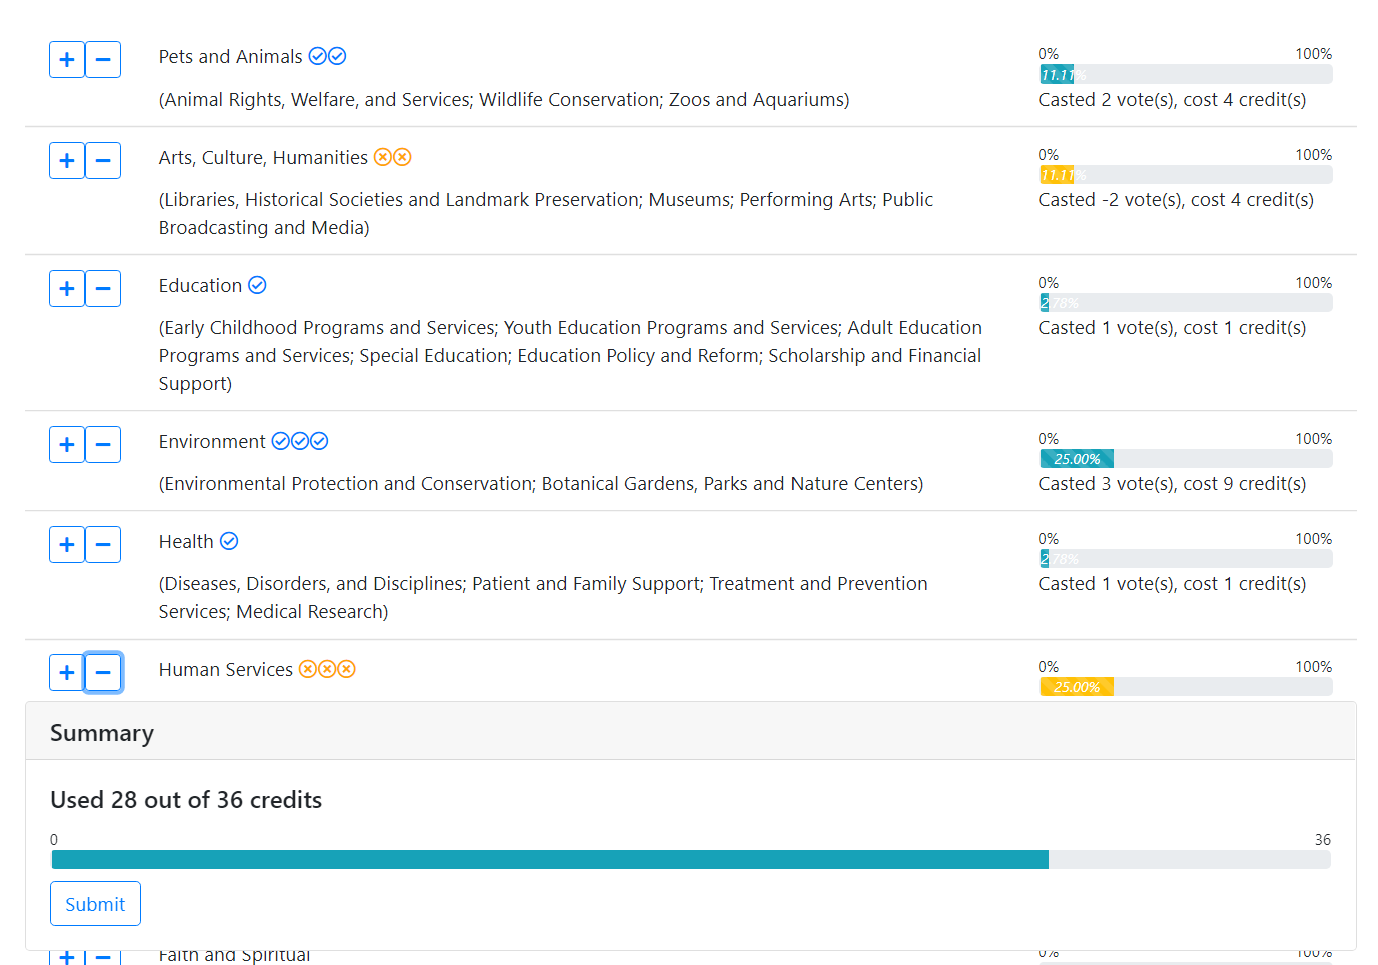
\includegraphics[width=0.7\textwidth, keepaspectratio=true]{content/image/qv-donation.png}
    \caption{
        The QV voting interface used in the experiments. 
        We omitted the prompt in this figure.
        After mutiple iterations, 
        the interface allows participants to vote, 
        with real time feedback of how the votes allocats. 
        The progress bar implementation 
        were inspired by knapsack voting interface by \cite{goel2015knapsack}.
    }
    \label{fig:qv_donation}
\end{figure}

The QV interface (\Cref{fig:qv_donation}) added more visual information than the pretest interface to reduce the participant's cognitive load. In this figure, we omitted the prompted on top of the page. The body section is the voting panel that contained all options to vote. To the left of each option, participants vote using the plus and minus buttons. Buttons were automatically disabled if the number of voice credits remaining does not permit the next vote of that item. Instead of cluttering information beneath each option in QV, we presented the information about that option to the left-hand side. We provided participants a bar right of the option, which showed the proportion of voice credits used to that option with text associated with the visual. We changed the color for the icons for ``for'' and ``against'' votes to improve accessibility. We floated the summary panel to the bottom of the page to ensure visibility. In the summary panel, we displayed a progress bar that showed the number of voice credits the participants have and have not used.\par

%% Old draft text
% % Experiment overview
% We designed the first experiment as a between within-subject study
% consisting of Likert survey, QV, and a donation task,
% to answer research questions one and three. 
% Participants were recruited from Amazon Mechanical Turk (MTurk).
% The Likert Group received \$0.75 
% while the QV and Likert Group received \$1.75 
% when participants completed the study.
% In this section, 
% we detailed our experiment design.

% The goal of a between within-subject study is to
% understand how within-subject does a survey tool
% aligns with one's true preference.
% To compare QV and Likert, 
% these results, 
% the difference between the survey tool and one's preference, 
% were then compared across groups of participants.

% %The donation task. Why?
% In order to figure out 
% how QV and Likert surveys 
% represent an individual's true preferences,
% we ask participants to complete a survey
% and donate to a charity.
% Our goal is to see 
% whether a participant's donation behavior is similar to 
% the attitudes they stated in the survey.
% There are multiple reasons
% why we designed a donation task.
% First, donation tasks are easily relatable
% given that they occur in real life and
% and monetary behaviors are direct and imaginable.
% Second, donations are simple to conduct,
% even on a large scale.
% Third, donation tasks appeared in many experiments 
% \cite{Xiao2019, benz2008people, gendall2010effect} 
% as an effective indicator of participants' behavior.
% Fourth, donating is a behavior containing
% complimentary and homogenous choices and
% where each of the options is independent.
% It is a clear example of choosing one out of $K$ in real life.

% \begin{figure}[htpb]
%     \centering
%     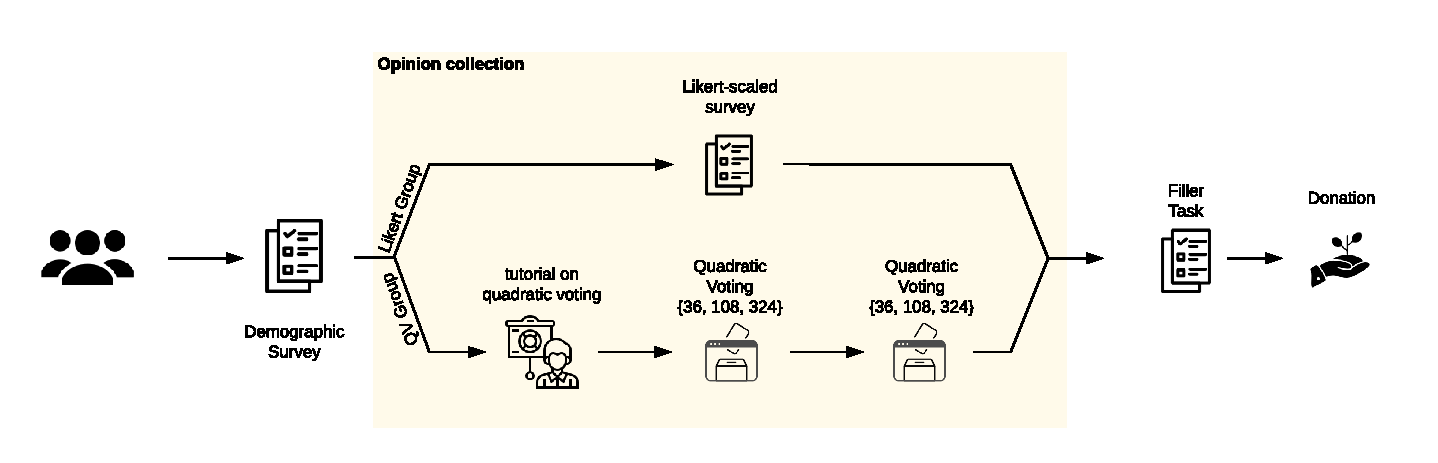
\includegraphics[width=\textwidth, keepaspectratio=true]{content/image/exp1_flow.pdf}
%     \caption{
%         Experiment one conducted between and within subjects. Participants were divided into two groups. Participants that took the upper path are the Likert Group, who expressed attitudes of various social causes through a five-point Likert Survey. The alternative is the QV group who replied attitudes through two QV surveys, each with a different combination among the three possible votes: $36$, $108$, or $324$ credits.
%     }
%     \Description[Image describing the flow for experiment 1]{Image describing the flow for experiment 1}
%     \label{fig:exp1_image_flow}
% \end{figure}

% At a high level, 
% we summarize the experiment flow 
% in Graph \ref{fig:exp1_image_flow}.
% The experiment consisted of four steps:
% To begin the experiment, 
% participants filled out the demographic survey.
% Based on the demographics,
% participants completed one form of opinion collection,
% highlighted as the yellow box
% in Graph \ref{fig:exp1_image_flow}.
% After that, 
% participants filled out another survey,
% the distraction survey,
% to divert their attention before they complete the final task.
% The final task asked participants to donate.
% Now we explain each section in detail.

% Before starting the experiment,
% participants were told that 
% this study aims to understand their opinions 
% toward social causes and will be asked to complete a donation task.
% During the demographic survey, 
% we collected the participant's gender, ethnicity, age range, household income level, 
% education level, and current occupation.
% Based on the age and education level,
% we divided participants into seven groups
% and made sure each group contained the same distribution
% as the US 2019 census.
% These seven groups can be further categorized as
% the Likert Group (Group 1) and the QV Group (Group 2 to 7).
% The Likert Group, shown as the upper path in the shaded area of Graph \ref{fig:exp1_image_flow}, 
% revealed their opinion using a Likert survey.
% The QV Group, shown as the lower path in the shaded area of Graph \ref{fig:exp1_image_flow}, 
% revealed their opinions by completing two QVs, each with different numbers of voice credit.
% We divided the QV Group into six subgroups
% to answer research question three, 
% which is whether the number of voice credits impacts the outcome.
% These two voice credits that participants experience 
% are drawn from three possible values: $N \times O$, $N^{1.5} \times O$, $N^2 \times O$, 
% where $N$ is the number of options in the survey, 
% and $O$ is the number of levels, 
% excluding neutral on the Likert survey. %not sure if this is clear
% In our case, with nine options ($N=9$) and
% used a five-point Likert survey ($O=4$), 
% the three values would be $36$, $108$, and $324$.
% With these three possible values, 
% we choose two for each of the six subgroups.

% In the Likert group, 
% the survey looks identical to a typical five-point Likert survey.
% We assume participants have prior knowledge in Likert surveys.
% Participants were presented with the nine societal causes, 
% and were asked the importance each of these causes: 
% With options ranging from ``Very important'' to ``Very Unimportant.''

% In the QV group, 
% participants were asked to watch 
% a prerecorded tutorial video of QV's concept 
% and how to operate the QV interface.
% Participants are granted unlimited time 
% to interact with a demo QV interface. 
% This process is demonstrated as 
% ``tutorial on quadratic voting'' 
% in Graph \ref{fig:exp1_image_flow}.
% To ensure that participants paid attention to the video and understood QV, 
% they were asked to answer at least three of the five multiple-choice questions 
% correctly to continue with the survey.
% Once participants passed the quiz, 
% participants will be given voice credits of either 36, 108, or 324.
% They will vote in QV using these voice credits 
% with the nine options identical to those in the Likert Group.
% Participants would repeat this action using a different set of voice credits.
% These two QVs are shown as two QV icons in Graph \ref{fig:exp1_image_flow}.

% After both groups of participants completed their surveys in the opinion collection stage, 
% they finish a short answer question
% that allowed them to express their thoughts 
% related to another set of societal issues.
% These societal issues are unrelated in the previous stage,
% and are designed to distract participants.
% We do not want participants to connect their survey responses
% to interfere with their behaviors during the donation task.

% Finally, 
% we ask participants to perform a donation in the final stage.
% This task presented nine organizations,
% each referring to one of the nine societal causes
% that we listed during the opinion collection phase.
% Participants can donate 
% any amount to any of the listed organizations
% without exceeding a total of 35 dollars.
% To ensure incentive compatibility, 
% participants do not donate imaginatively.
% Participants are aware that every one in 70 participants would win 35 US dollars.
% Assuming winning the 35 US dollars, 
% the participants were asked 
% if they would want to donate some money 
% to any of the nine charity groups.
% Participants are also aware that 
% they keep the remaining amount of undonated money 
% if they win the lottery.
% Further, participants are aware that 
% the research team will match one dollar to each one dollar 
% they donated to an organization.
% \tc{We need to justify why we matched}
% This setup means the donation carried an underlying cost.

% To minimize the difference across groups in the study, 
% we use the same prompt across Likert survey, QV, and the donation task.
% We explicitly tell the participants that 
% there are limited resources in the society, 
% and people have different preferences 
% in how resources should be allocated and ask the participants, 
% ``What societal issues need more support?''

% To ensure that the nine societal causes 
% covered a broad spectrum of categories.
% We used the categorization of charity groups on Amazon Smile, 
% a popular donation website that has accumulated over 100 million dollars of donations, 
% as our topics of the societal causes.
% The categories include:
% \begin{enumerate}[label={},leftmargin=\parindent]
%     \item (1) Pets and Animals
%     \item (2) Arts, Culture, and Humanities
%     \item (3) Education
%     \item (4) Environment
%     \item (5) Health
%     \item (6) Human Services
%     \item (7) International
%     \item (8) Faith and Spiritual
%     \item (9) Veteran
% \end{enumerate}
% Within each of these categories, 
% we select one charity organization from Amazon Smile 
% as the representation of the subject matter used in the donation task.

% \subsection{System Design}
% We use Python Flask for the back-end, Angular for front-end, 
% and MongoDB for database storage to construct the voting system. 
% The experiment source code is publicly available \footnote{Not yet public}, 
% and so is the QV interface as a stand-alone repository \footnote{https://github.com/hank0982/QV-app}.

% \begin{figure}[htpb]
%     \centering
%     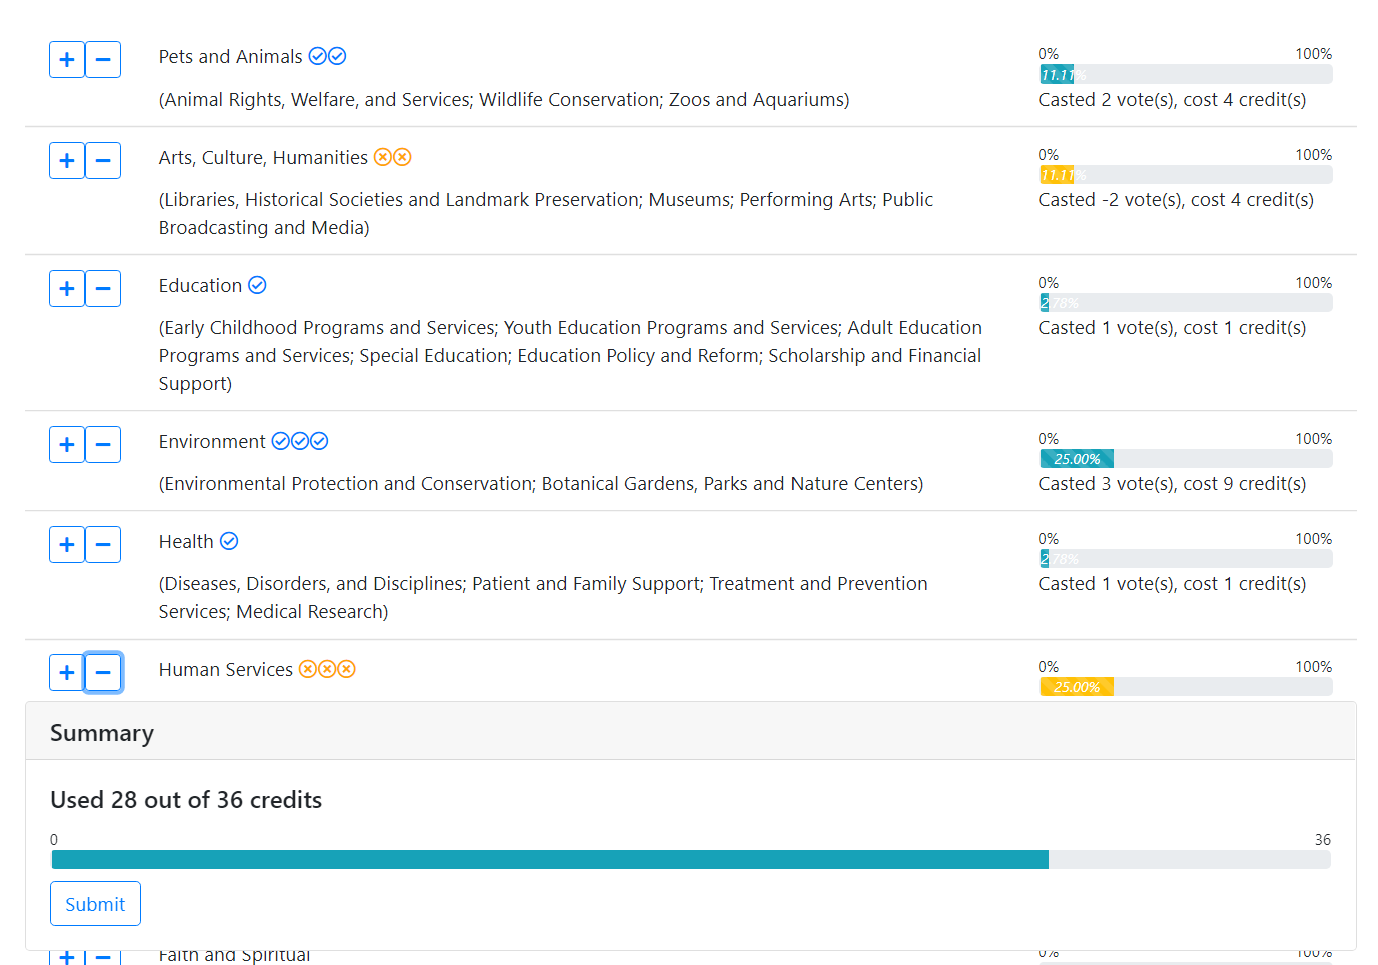
\includegraphics[width=0.7\textwidth, keepaspectratio=true]{content/image/qv-donation.png}
%     \caption{
%         The QV voting interface used across both experiments. 
%         We omit the prompt in this figure.
%         After mutiple iterations (details in the Appendeix), 
%         the interface allows participants to vote, 
%         with real time feedback of how the votes allocats. 
%         The progress bar implementation 
%         were inspired by knapsack voting interface by \textcite{goel2015knapsack}.
%     }
%     \label{fig:qv_donation}
% \end{figure}

% The QV interface, is shown in Figure \ref{fig:qv_donation}.
% The body section is the voting panel
% that contained all options to vote for.
% To the left of each option, 
% participants vote using the plus and minus buttons.
% Buttons are disabled 
% if the number of voice credits 
% does not permit the next vote.
% A bar on the right of the option 
% shows the proportion of voice credits 
% used to that option with text associated with the visual.
% The different colors and the icons 
% to the right of each option 
% exhibits the number of for or against 
% that currently devoted to an option.
% The summary panel always 
% floats at the bottom of the page 
% to ensure visibility.
% A progress bar shows the number of voice credits 
% that the participants have and had not used.\par